\documentclass[preprint,11pt,authoryear]{sigplanconf}

% The following \documentclass options may be useful:
%
% 10pt          To set in 10-point type instead of 9-point.
% 11pt          To set in 11-point type instead of 9-point.
% authoryear    To obtain author/year citation style instead of numeric.

\usepackage{amsmath}
\usepackage[T1]{fontenc}
\usepackage{graphicx}
\usepackage{color}

\begin{document}

\title{Verifying Interfaces in Ptolemy II}

\authorinfo{Ben Lickly}
           {University of California, Berkeley}
           {blickly@eecs.berkeley.edu}

\maketitle

\newcommand{\fixme}[1]{\textcolor{red}{FIXME: #1}}

\begin{abstract}
\end{abstract}

\section{Introduction/Motivation}
Component-based design allows for more efficient construction of large systems, by starting with existing components that have known behaviors.  In order to prove properties of the overall system, it is often enough to combine properties of the individual components.

Interface theories~\cite{interfaceTheories} specify what properties components require of their environments, as well as how and when they can be abstracted, composed, or refined.
\subsection{Motivation}
Often, interface theories have their precise semantics captured only in the English text of the works in which they are published.
Rather than reading these texts and performing the computations by hand, wee would like to automate these operations so that they can be checked (for some cases) by a computer.
Since the problem is undecidable in general, we accept having a partial algorithm that may return "unknown."

One key question is that of interface composition.  In component based verification, properties of the overall systems are proved by composing properties of the components, and the interface theories tell us how to make the compositions.

A typical example of where this type of tool would be useful would be in the early stages of system specification.
Different designers could specify certain aspects of components to built that they would guarantee.
This specification could be done much more quickly than building even a prototype component, but it would still be useful for specification.
This tool would then be able to check that these components can be composed.
If it happens that this requirement cannot be met, then the design must be reconsidered.
This may point to a fundamental design flaw, but it may also simply mean that some designers must provide stronger guarantees of what their components will do.

For example, say we have two components, as well as some abstractions that make up their interfaces, and be interested in the composition of those two interfaces.  One problem that might occur in this scenario is as follows: if the interfaces of the original components are too abstract, then the interfaces may not be composable.  In this case, the developer may need to come up with a more concrete interface, whose behavior is closer to the behavior of the realized component.  It would also be nice if we could algorithmically check whether interfaces were composable, making this process faster and less error-prone.

\section{Background/Related Work}
In~\cite{relationalInterfaces}, Tripakis et. al. propose a relational type of interface that can capture interactions between inputs and outputs.  This allows more complex behaviors to be captured, but it also means that working with the interface theory can be more difficult.

Here, we aim to build a system for automatically checking the satisfiability of such interfaces and to aid in composing them.  We choose to base our work on Ptolemy II~\cite{ptII}, an actor-based modeling tool that contains supports hierarchical compositions of heterogeneous components.

\fixme{Check emails from Stavros}
\section{Approach}
Create a domain for Ptolemy II that \dots

\subsection{Definitions}
We define a deterministic interface to be one for which the outputs are uniquely determined by the inputs (and the current state, if stateful) for all valid inputs.  Even though most of our real components may behave deterministically, our interfaces may be abstractions of this behavior, and thus they are often not deterministic.  Informally, we can discuss one interface being more deterministic (or more abstract) than another.

An interface $A=(X,Y,\phi_A)$ is \emph{more deterministic} than interface $B=(X,Y,\phi_B)$, if
\[
\phi_B \implies \phi_A \wedge \phi_A \not\implies \phi_B
\]
If we view the contract as simply specifying a relation between the inputs and the outputs, $R(\phi) \subseteq X \times Y$, then A being more deterministic than B simply means that
$R(\phi_A) \subset R(\phi_B)$


\subsection{Examples}
\begin{figure}[htbp]
\centering
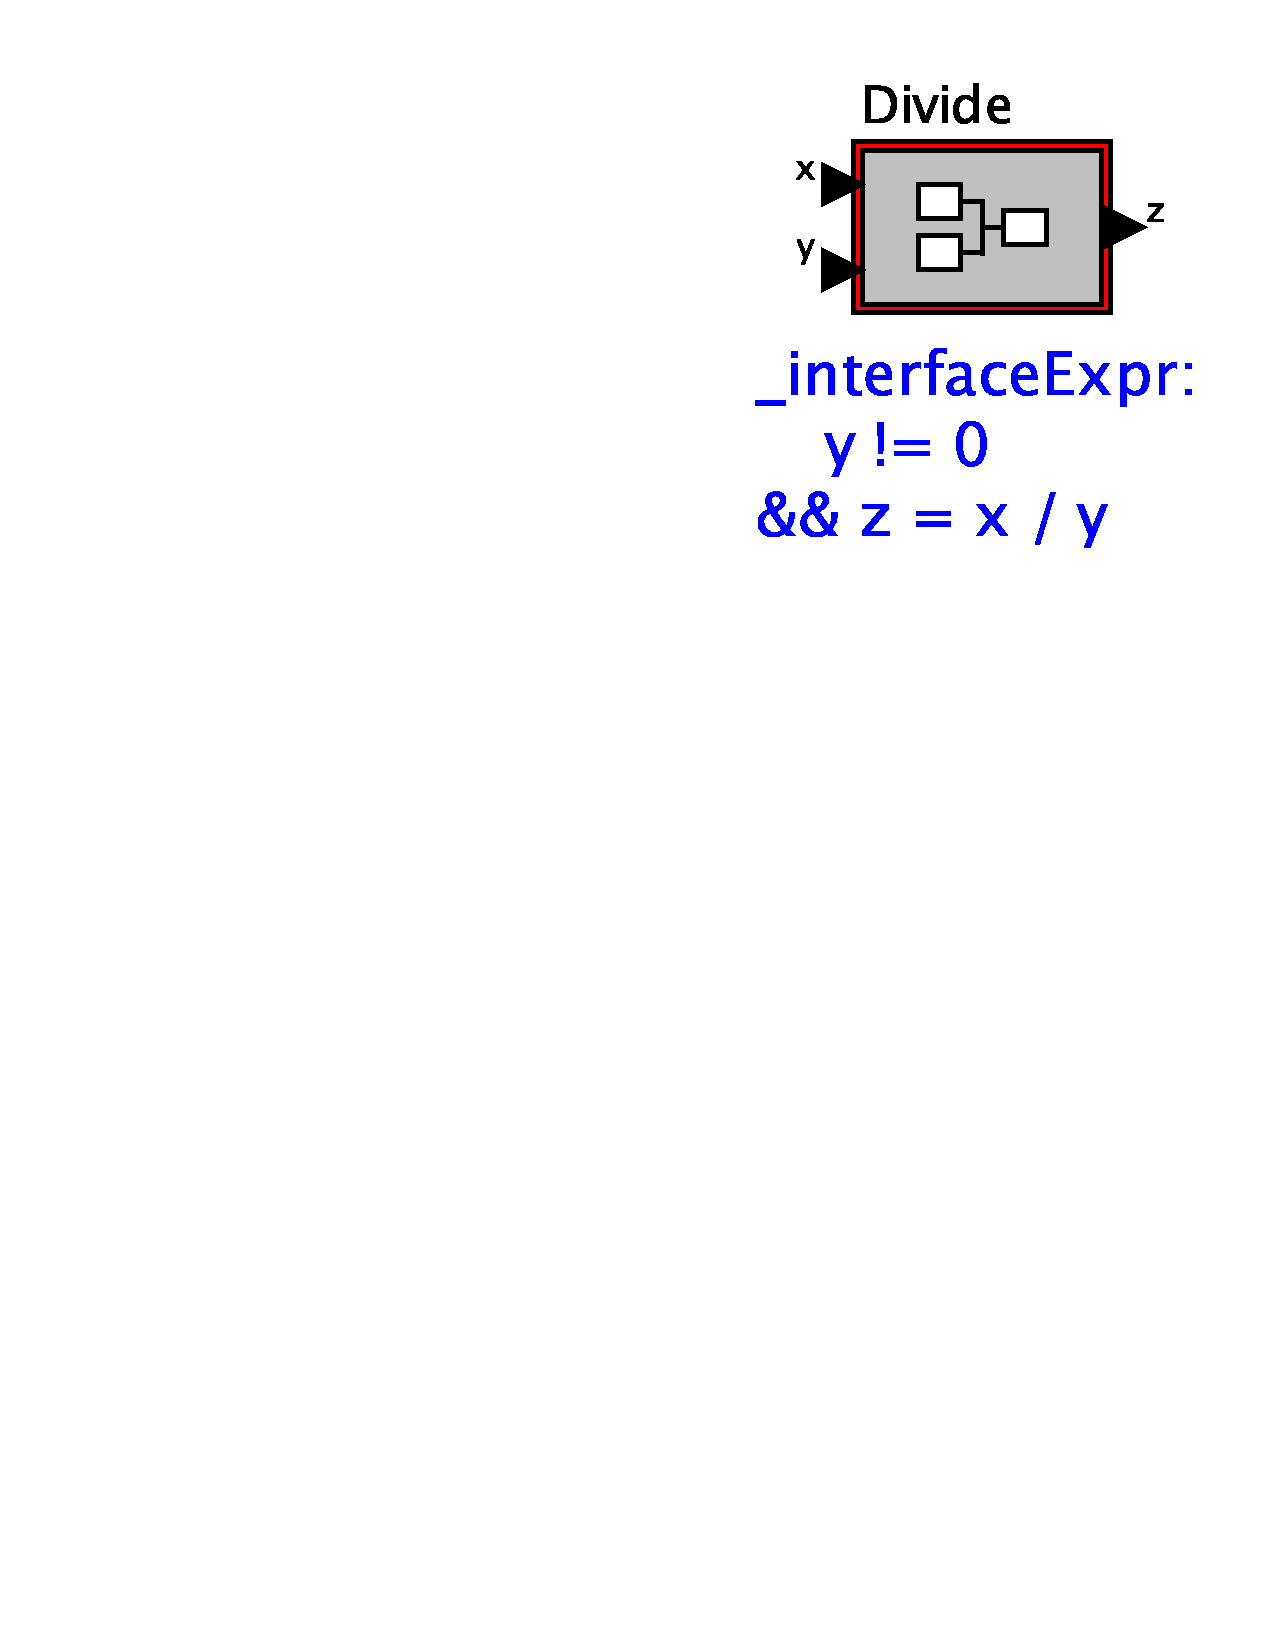
\includegraphics[width=\columnwidth]{figs/Divide2} 
\caption{An interface of a divider actor.}
\label{fig:divider}
\end{figure}

\begin{itemize}
	\item Valid composition with too abstract interfaces
	\item Invalid composition
\end{itemize}

\section{Solution}
Here, we add an interface to the Yices\cite{yices} SMT solver to the Ptolemy II\cite{ptII} project.
We do this through the use of a new Ptolemy~II director, called the \texttt{InterfaceCheckerDirector}, which checks for the validity of interfaces in the actors of a model.
We allow each actor in the model to be annotated with a parameter to specify its interface.
Here we supporting both native Ptolemy~II expressions, which have a C-like syntax, and LISP-style string expressions in the Yices input language.
The Ptolemy expressions must be boolean valued, with a true value meaning the interface is satisfied, and they are searched for by looking for parameters of actors named $\_interfaceExpr$.
The Yices inputs language interfaces require string-valued parameters names $\_interfaceStr$, and allow richer expressions to be used.
This is because the Yices input language supports quantifiers, which are absent in the Ptolemy expression language.

The details of the interface theory itself are encapsulated in the \texttt{RelationalInterface} class, allowing for different interface theories to be added later, although currently only the relational interface theory of~\cite{relationalInterfaces} is supported.
Interface theories themselves must handle cascade composition from one interface to another, parallel composition of two interfaces,
and feedback composition.  In cases where these compositions are not possible, the interface theory must throw an exception.
%FIXME: Make this true

\subsection{Examples}
Here are some examples of how to use the tool to check for model compatibility.

In the first example, the user wants to compose two components.  In order to do that, he must first check that the interfaces are composable.  The first component takes an absolute value, and the second component takes the inverse of its input.

\subsubsection{Interface Error}
\begin{figure}[htbp]
\centering
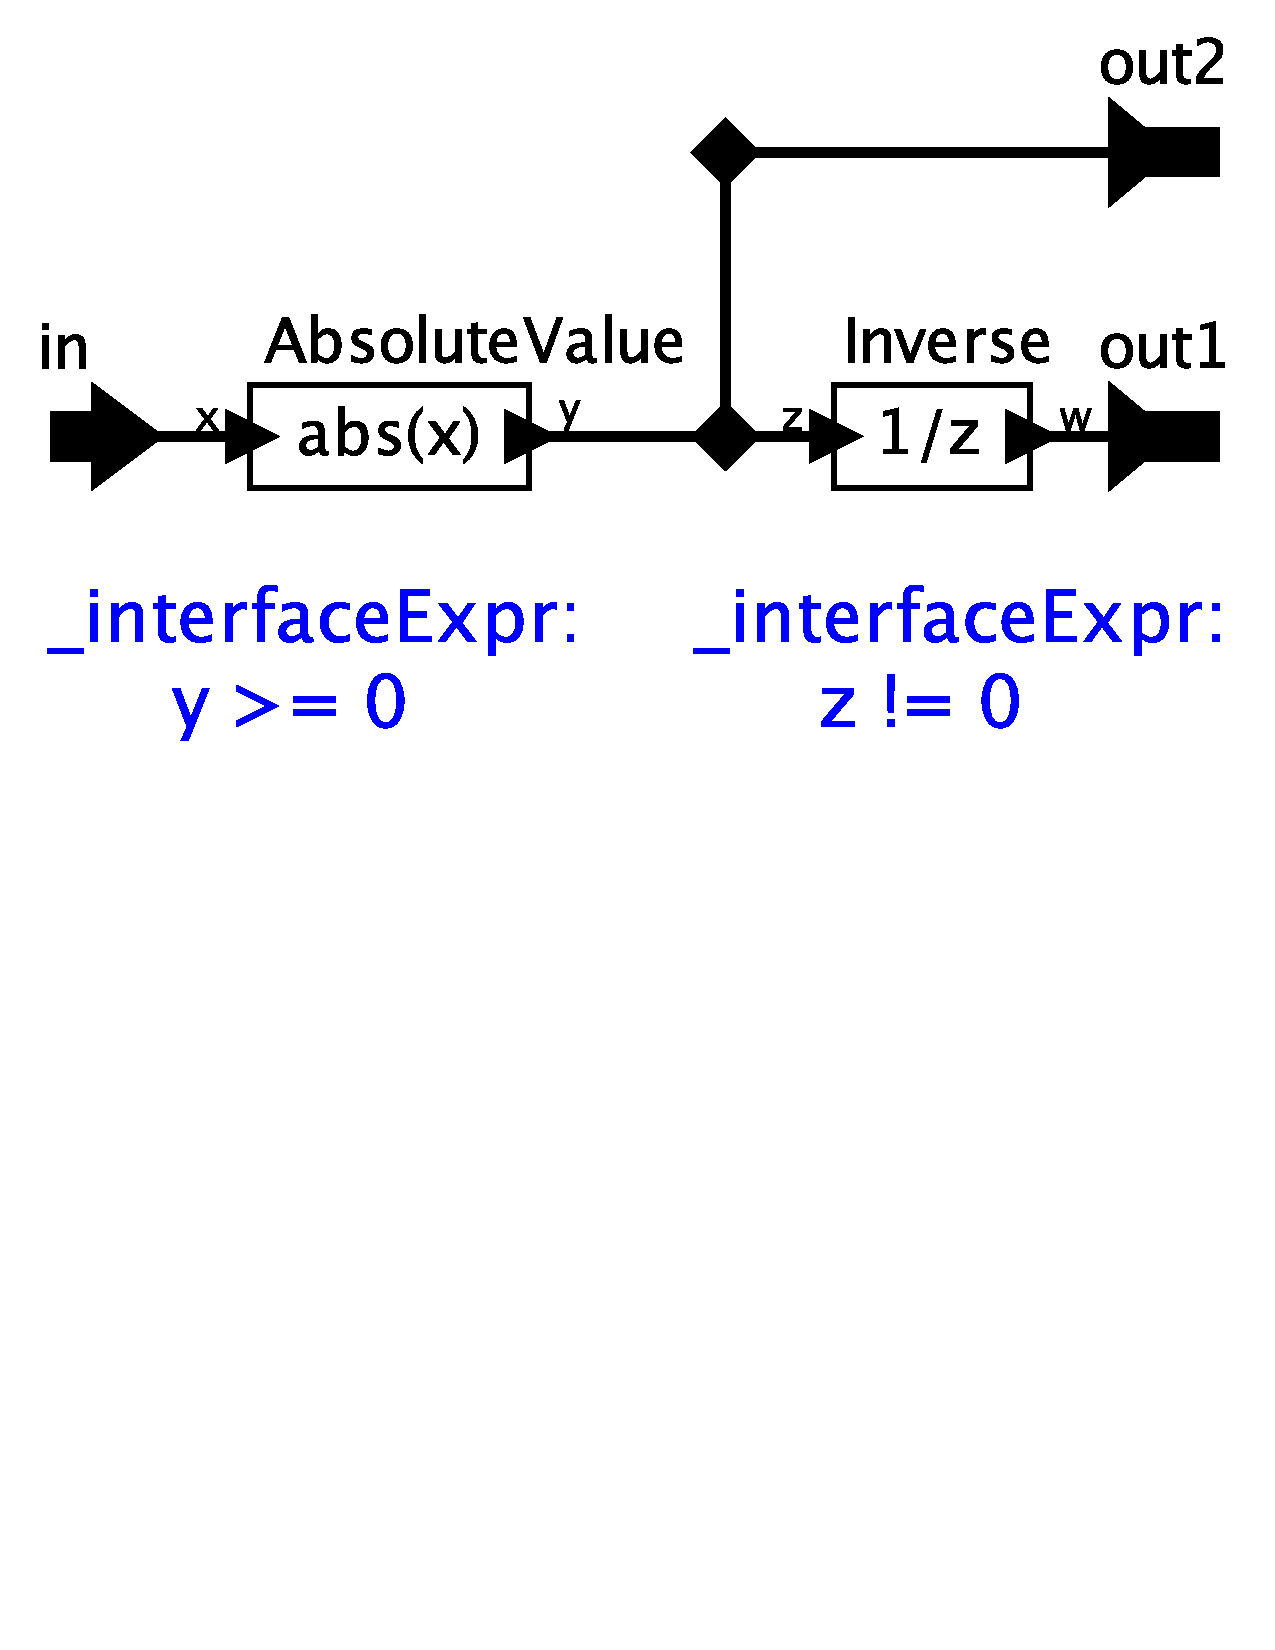
\includegraphics[width=\columnwidth]{figs/absoluteError}
\caption{An error in interface specification.}
\label{fig:absoluteError}
\end{figure}

In this example, interfaces are being used to prove safety properties of the system, so any abstractions must be overapproximations.  In the first attempt, the user choses the contract
\[
y >= 0
\]
for the absolute value.  <!--If we consider this formula as a relation, it contains all pairs of inputs and outputs such that the input is not simultaneously zero with the output non-zero.-->  Clearly this is an overapproximation of absolute value, since it doesn't take into account the input to the actor.
For the inverter, the user choses the contract
\[
x \ne 0
\]
to capture the restriction that we cannot divide by zero.  Since this contract does not specify the output value, it too is an abstraction that overapproximates.

\begin{figure}[htbp]
\centering
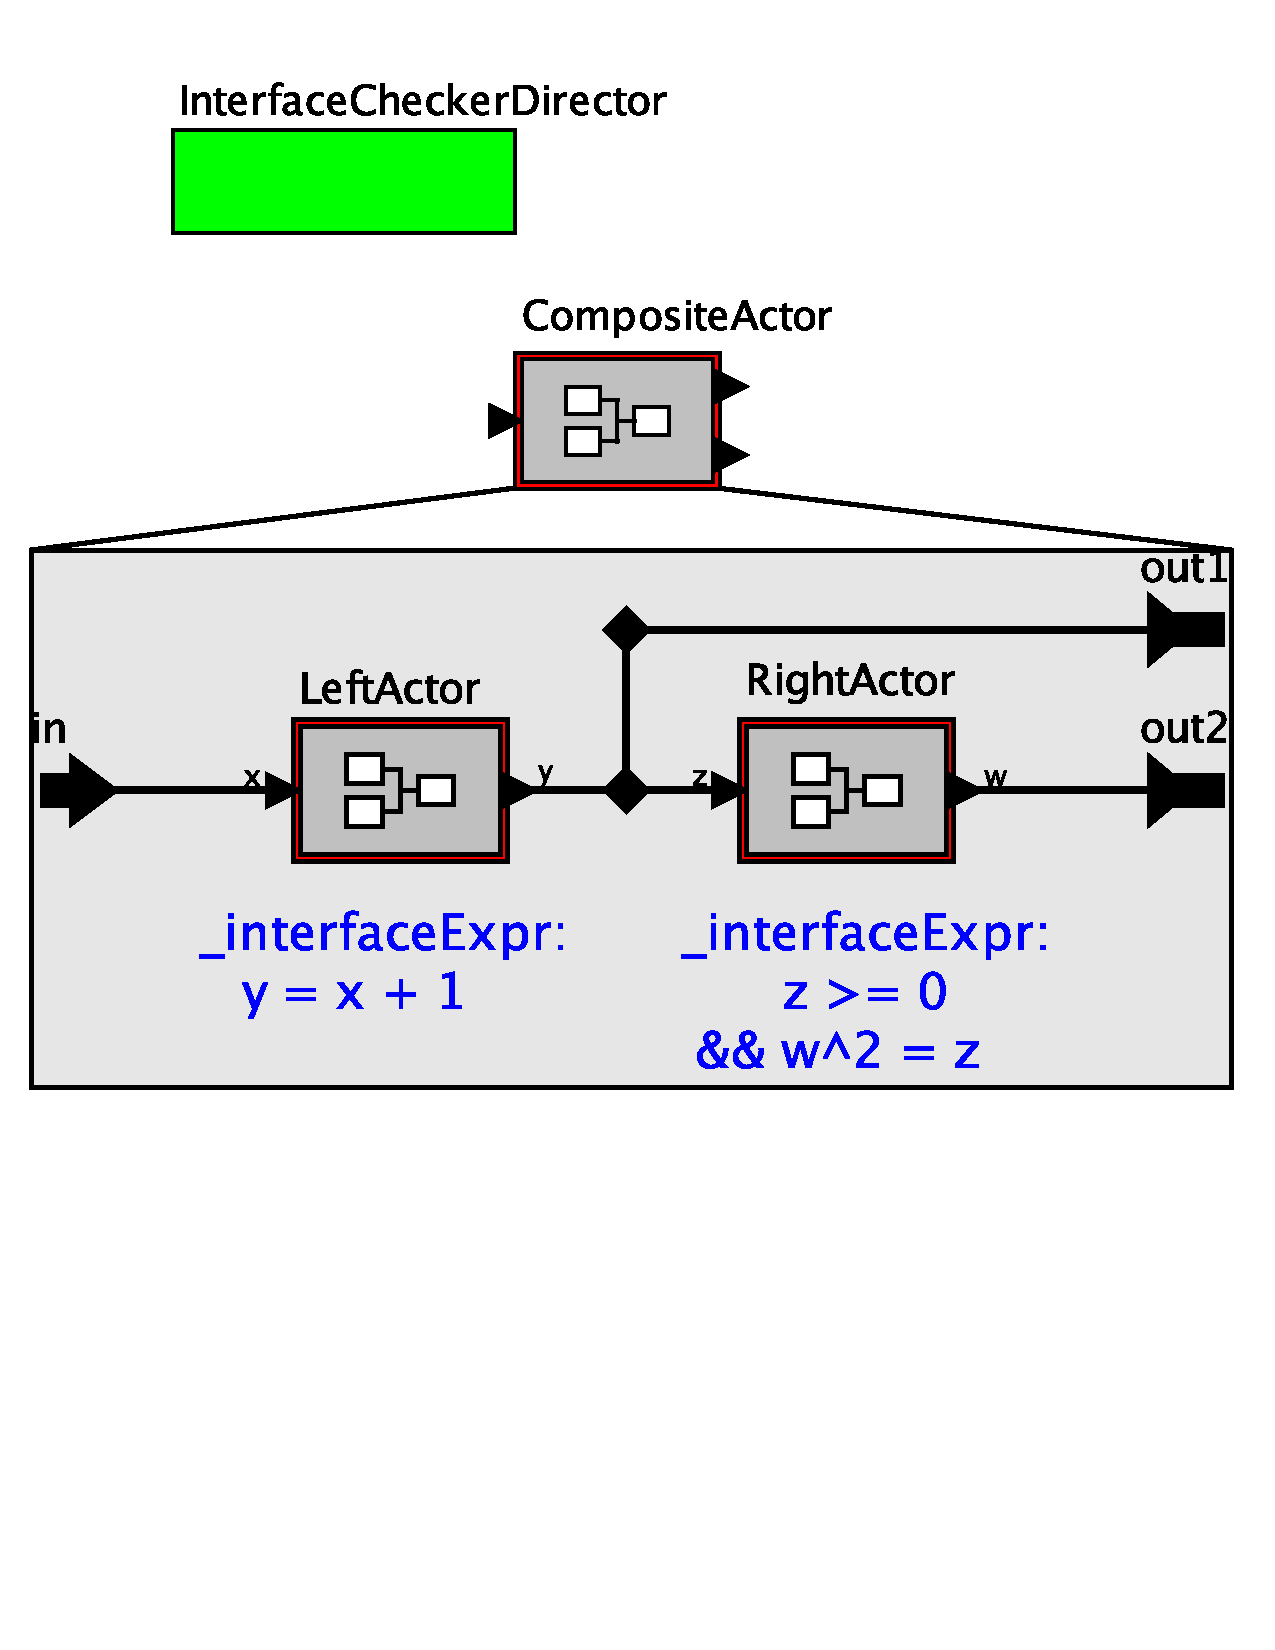
\includegraphics[width=\columnwidth]{figs/cascadeComp} 
\caption{A composite actor formed by the cascade composition of two contained actors.}
\label{fig:cascadeComp}
\end{figure}

\begin{figure}[htbp]
\centering
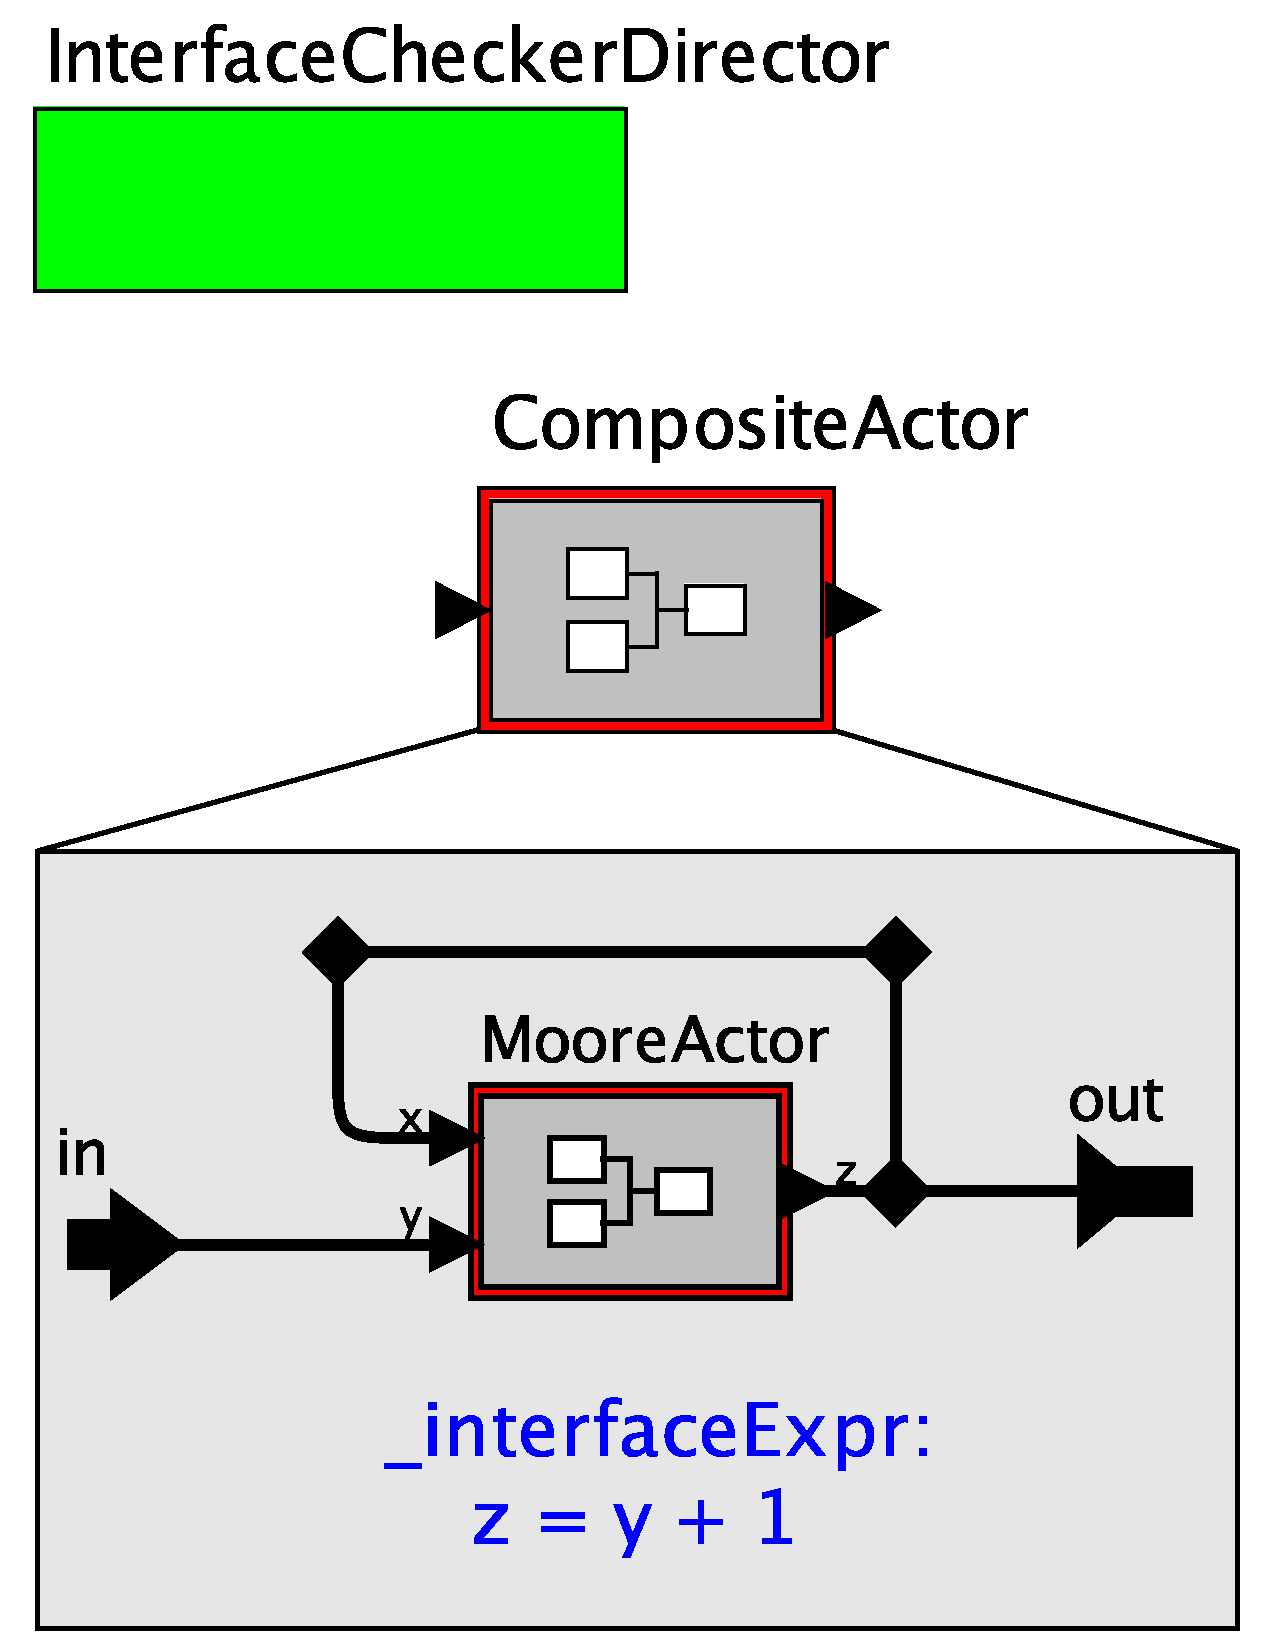
\includegraphics[width=\columnwidth]{figs/feedbackComp} 
\caption{A composite actor formed by adding feedback to its contained actor.}
\label{fig:feedbackComp}
\end{figure}

In this case, if we run our tool, we can see that the resulting composition interface is not valid.  Intuitively, this is because there is no input to the first interface such that we can guarantee its output will not be zero.  Since these interfaces do not compose, we need to make them more concrete.

\begin{figure}[htbp]
\centering
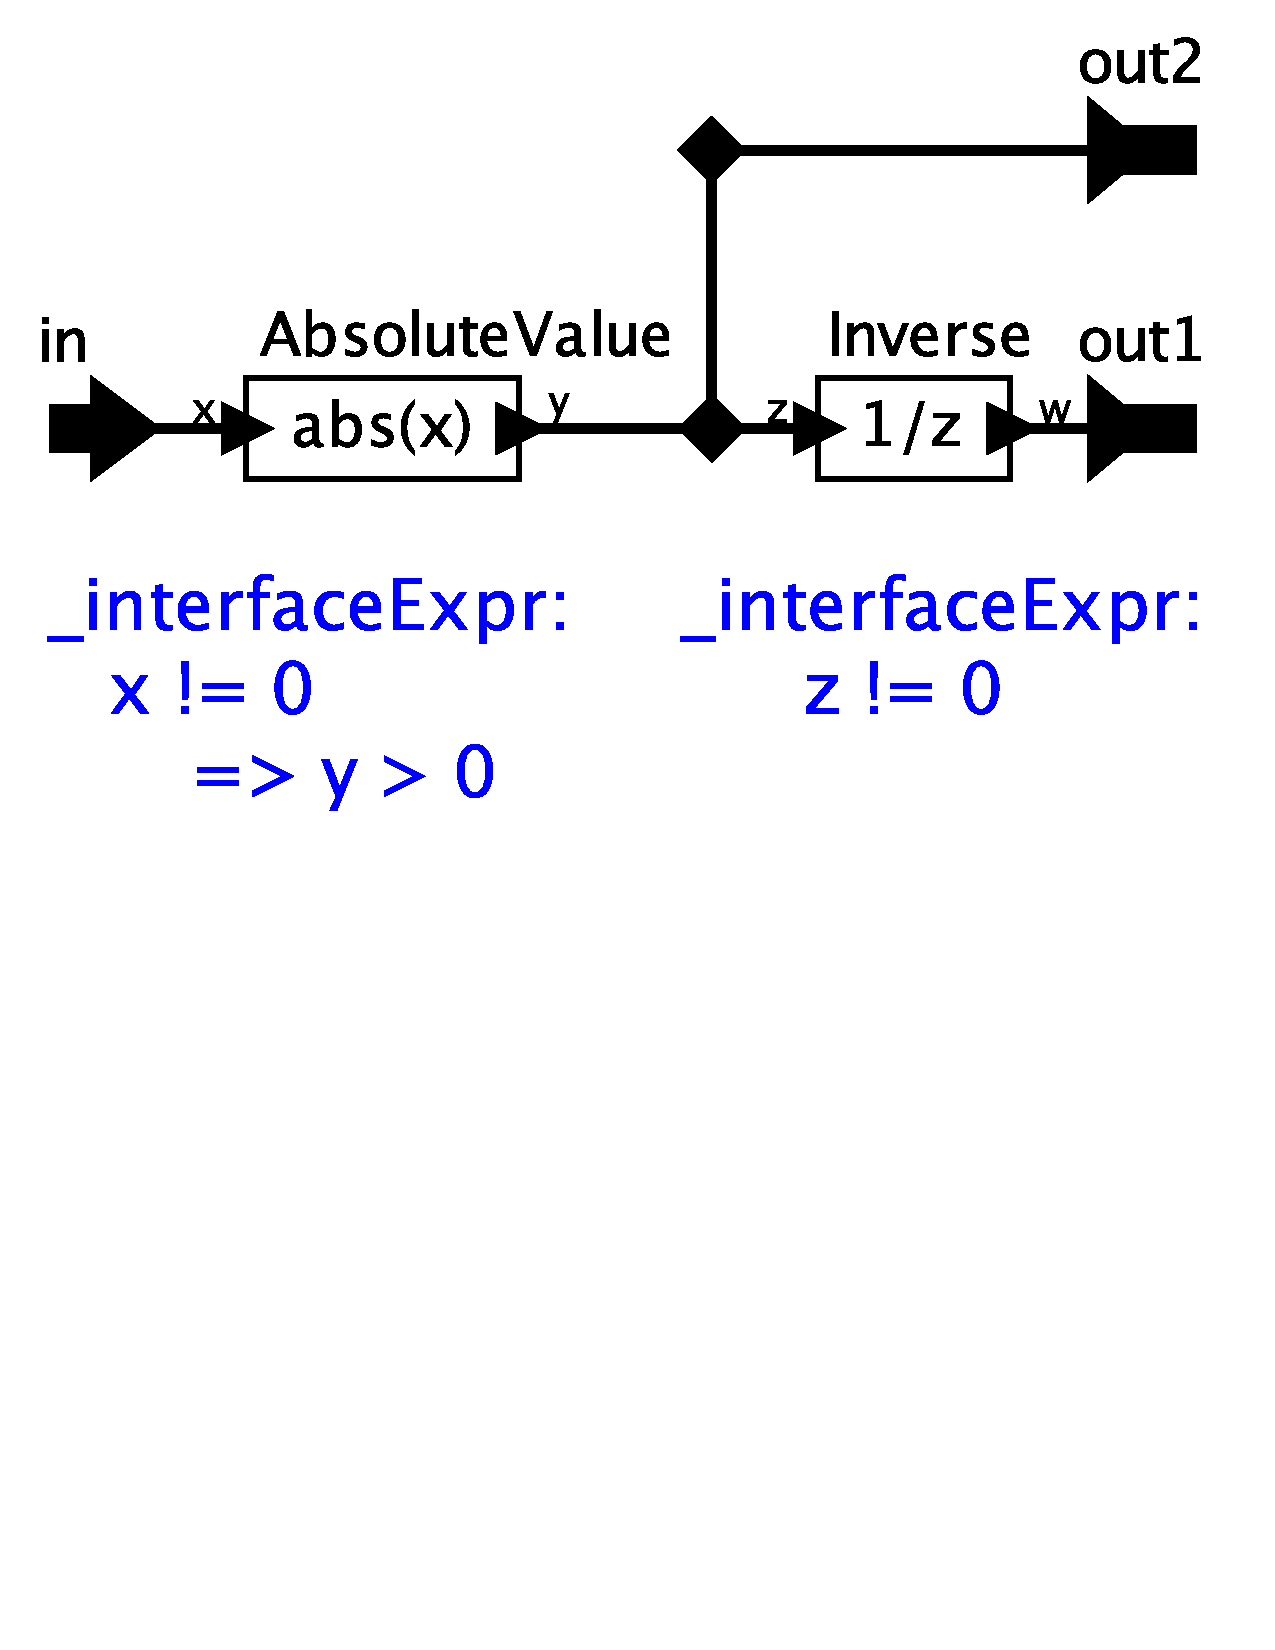
\includegraphics[width=\columnwidth]{figs/absoluteCorrected}
\caption{A fixed interface specification.}
\label{fig:absoluteCorrected}
\end{figure}

A second attempt at defining the component interfaces for this same model is given in Figure%~\ref{}. %FIXME
Here, the interface of the inverter is unchanged, but the interface for the absolute value is changed to
\[
a != 0 \implies y > 0
\]
P.S. Let's try an example with \[ a >= 0 \implies y = a\] or even \[a >= 0 \implies y = a  \wedge a < 0 \implies y = -a\]

\subsubsection{Component Error} \label{sec:componentError}
\begin{figure}[htbp]
\centering
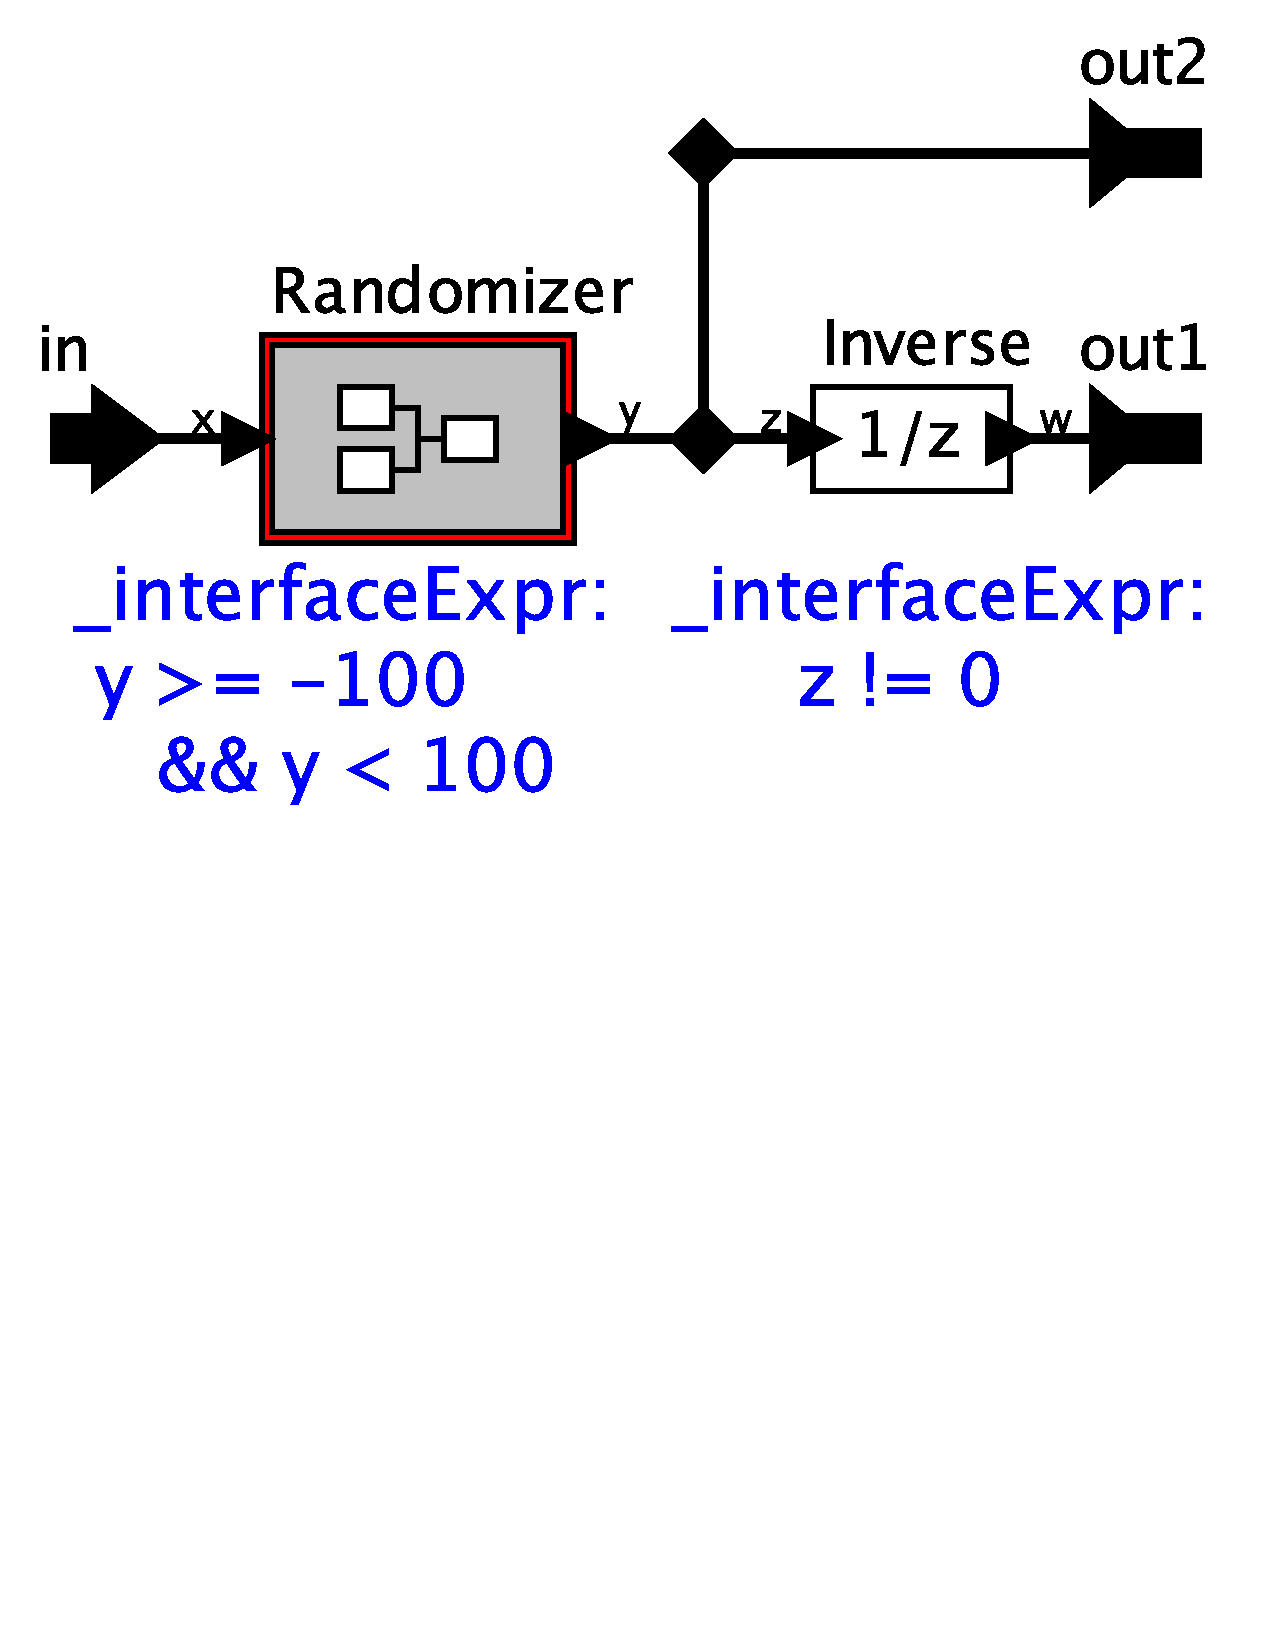
\includegraphics[width=\columnwidth]{figs/Randomizer}
\caption{An error in component composition.}
\label{fig:randomError}
\end{figure}

Consider another example in which the first component produces a random value in the range $[2^{-31}, 2^{31}-1]$, and the second component is the same as before.
The most deterministic valid constraint that the user can use for the first component would be
\[
y \ge 2^{-31} \wedge y \le 2^{31}-1
\]

In this case, running our tool will tell us that these components cannot be composed.
This time, however, this is not caused by the interfaces being too abstract; in fact, they are maximally deterministic.
The reason why we cannot compose these interfaces is that these components cannot be safely composed.

\section{Conclusion}
Here, we have presented an infrastructure for verifying interfaces of components in Ptolemy~II, our actor based modeling tool.
Our work currently checks for the validity of interfaces, and whether interfaces can be composed with each other.
In addition, our work is the first to present a general infrastructure for interfaces in Ptolemy~II.

As a general infrastructure, there are many possible extensions.
One would be the addition of run-time checks to test that the values produced by the implementation conform to the interfaces.
This could be a check of both the implementations and the interfaces.
Interestingly, these checks could even have predictive power.
For example, take the example from Section~\ref{sec:componentError} with the first component changed so that it adds the random jitter to its input, rather than produce a random number by itself.
Then any run using a value within the jitter of zero would be flagged as incompatible, even if that particular run caused no error in any component.

Another possible addition would be to allow a model builder to specify the interface of a composite and check that that specification
were valid.
In this case, it would be acceptable for the user-specified interface to be more abstract than the inferred interface, since the model designer is free to abstract away details that he or she knows to be irrelevant.
Thus, the automated check would verify that the inferred interface refine the specified interface.
Interface theories specify formally what it means for one interface to refine another, like they do for composition, but informally, it simply means that the new interface can be used in place of the refined interface.

There are many other possible, more long term extensions to this work, such as guessing and learning interfaces of atomic components by observing runtime behavior, or checking statically that the Java definition of an actor meets its interface.
% Or more...

Finally, one of the most important uses of this tool is for developing new interface theories.
Using this tool allows for rapid experiment with various interfaces, storage of examples in an executable form, and checking of hand proved results.
In addition, the architecture encourages swapping out of one interface theory for another, which should make it easy to experiment with new theories altogether.


\acks

Acknowledgments, if needed.

% We recommend abbrvnat bibliography style.

\bibliographystyle{abbrvnat}
\bibliography{refs}

\end{document}
